% -*- LaTeX -*-
% -*- coding: utf-8 -*-
%
% michael a.g. aïvázis
% california institute of technology
% (c) 1998-2012 all rights reserved
%

%-----------------------------------

\section{components}
\subsection{overview}

%-----------------------------------
\begin{frame}
%
  \frametitle{Components and protocols}
%
  \begin{itemize}
%
    \item a design pattern that enables the assembly of applications out of interchangeable
      parts, under the control of the {\em end user}
      \begin{itemize}
      \item {\em protocols} are abstract specifications of application requirements
      \item {\em components} are concrete implementations that satisfy requirements
      \end{itemize}
%
    \item inversion of control:
      \begin{itemize}
      \item the binding of implementations to specifications happens at runtime, under the
        control of the end user
      \end{itemize}
%
    \item the user 
      \begin{itemize}
      \item controls the application state through configuration files, the user interface, the
        command line
      \item specifies components using simple URIs
      \end{itemize}
%
    \item the goal is to isolate contributors from each other as much as possible, and provide
      a coherent and usable strategy for composing non-trivial applications
%
  \end{itemize}
%
\end{frame}

%-----------------------------------
\begin{frame}
%
  \frametitle{A non-trivial example}
%
  \begin{itemize}
  \item {\tt gauss}: an extensible numeric integration package
    \begin{itemize}
      \item specify protocols and components
      \item identify the configurable state
      \item implement component behavior in terms of the specified protocols
    \end{itemize}
  \end{itemize}
%
  \begin{figure}
    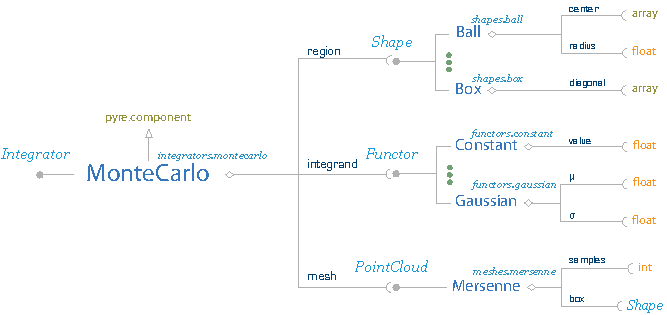
\includegraphics[scale=1.0]{figures/montecarlo.pdf}
  \end{figure}
%
\end{frame}

%-----------------------------------

\subsection{implementation}

%-----------------------------------
\begin{frame}
%
  \frametitle{Implementation strategy}
%
  \begin{itemize}
%
  \item key abstractions:
    \begin{description}
    \item[functor:] encapsulation of a function in a class; our integrands will be functors
    \item[shape:] a spatial domain; we will use these to specify the region of integration
    \item[mesh:] a discretization of the domain of integration; meshes provide the locations at
      which we sample integrands
    \item[integrator:] the implementation of a particular integration algorithm
    \end{description}
%
  \item each one of these will turn into a {\em protocol}
    \begin{itemize}
    \item that spells out all the obligations imposed on concrete realizations
    \end{itemize}
%
  \item {\em components}
    \begin{itemize}
    \item must provide concrete implementations of all the obligations
    \item specify their public state: what can be delegated to the end user
    \end{itemize}
%
  \end{itemize}
%
\end{frame}

%-----------------------------------
\begin{frame}
%
  \frametitle{Package layout}
%
  \begin{itemize}
%
  \item use the names of the abstractions to determine the directory layout
%
    \begin{columns}[t]
%
      \begin{column}{0.5\textwidth}
        \begin{figure}
          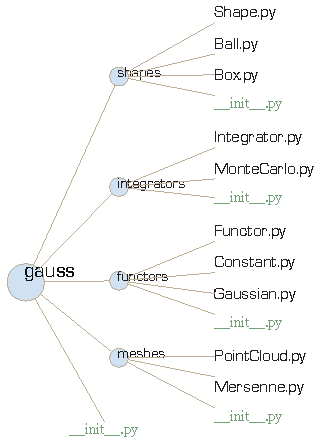
\includegraphics[scale=0.70]{figures/layout-files.pdf}
        \end{figure}
      \end{column}
%
      \begin{column}{0.5\textwidth}
        \begin{figure}
          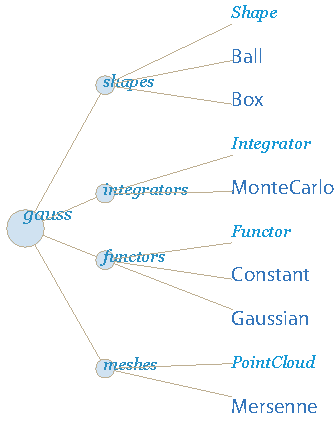
\includegraphics[scale=0.70]{figures/layout-namespace.pdf}
        \end{figure}
      \end{column}
%
    \end{columns}
%
  \item which affects the default {\em namespace} layout
%
  \end{itemize}
%
\end{frame}

%-----------------------------------
\begin{frame}
%
  \frametitle{The {\tt Shape} protocol}
%
  \vskip -1em
  \begin{itemize}
  \item in {\tt gauss/shapes/Shape.py}
    \python{firstnumber=9, linerange={9-31}}{listings/shape.py}
  \end{itemize}
%
\end{frame}

%-----------------------------------
\begin{frame}
%
  \frametitle{The {\tt Integrator} protocol}
%
  \vskip -1em
  \begin{itemize}
  \item in {\tt gauss/integrators/Integrator.py}
    \python{firstnumber=9, linerange={9-29}}{listings/integrator.py}
  \end{itemize}
%
\end{frame}

%-----------------------------------
\begin{frame}
%
  \frametitle{The {\tt MonteCarlo} integrator}
%
  \vskip -1em
  \begin{itemize}
  \item in {\tt gauss/integrators/MonteCarlo.py}
    \python{firstnumber=19, linerange={19-45}, basicstyle=\tt\tiny}{listings/montecarlo.py}
  \end{itemize}
%
\end{frame}

%-----------------------------------

\subsection{configuration}

%-----------------------------------
\begin{frame}
%
  \frametitle{User configuration}
%
  \cfg{firstnumber=7, linerange={7-23}, xleftmargin=4em}{listings/gauss.cfg}
%
\end{frame}

% end of file
